% Copyright (c) 2026 CorrectBrain
% SPDX-License-Identifier: MIT

\PassOptionsToPackage{dvipsnames,svgnames,x11names}{xcolor}
\documentclass[tikz,border=8pt]{standalone}
\usetikzlibrary{arrows.meta,positioning,calc,shapes,shadows,decorations.pathmorphing,shapes.geometric,backgrounds,decorations.markings,decorations.pathreplacing,decorations.text,fit,shapes.misc,shapes.arrows,matrix,bending,3d,chains,intersections,shapes.symbols,svg.path,shapes.multipart,snakes,shapes.callouts,angles,quotes}
\providecolor{gold}{RGB}{212,175,55}
\providecolor{silver}{RGB}{192,192,192}
\providecolor{bronze}{RGB}{205,127,50}
\providecolor{darkblue}{RGB}{0,0,139}
\providecolor{lightblue}{RGB}{173,216,230}
\providecolor{darkgreen}{RGB}{0,100,0}
\providecolor{lightgreen}{RGB}{144,238,144}
\providecolor{darkred}{RGB}{139,0,0}
\providecolor{navy}{RGB}{0,0,128}
\providecolor{skyblue}{RGB}{135,206,235}
\providecolor{beige}{RGB}{245,245,220}
\providecolor{cream}{RGB}{255,253,208}
\usepackage{amsmath}
\usepackage{amssymb}
\usepackage{fontawesome5}
\usetikzlibrary{fadings,shadows.blur,patterns,patterns.meta}

% --- DEFINED COLORS ---
\definecolor{cdncolor}{RGB}{103, 58, 183}    % Deep Purple
\definecolor{svgcolor}{RGB}{0, 150, 136}     % Teal
\definecolor{htmlcolor}{RGB}{230, 81, 0}     % Orange
\definecolor{codebg}{RGB}{40, 44, 52}        % Dark Gray for code
\definecolor{codetext}{RGB}{171, 178, 191}   % Light Gray for code
\definecolor{highlight}{RGB}{229, 192, 123}  % Yellow highlight
\definecolor{codeblue}{RGB}{97, 175, 239}
\definecolor{codegreen}{RGB}{152, 195, 121}

\begin{document}
\begin{tikzpicture}[
    % --- STYLES ---
    codebox/.style={fill=codebg, rounded corners=6pt, text=codetext, font=\ttfamily\small, inner sep=10pt}
]

% =========================================================================
% 1. GLOBAL CANVAS BOUNDING BOX & HEADERS
% =========================================================================
\fill[white] (-18, -21.0) rectangle (18, 15.5);

% Main Title & Subtitle
\node[font=\Huge\bfseries, text=black!80] at (0, 14.0) {The Architectural Isolation of SVG Assets};
\node[font=\Large\color{black!60}] at (0, 13.0) {How an independent \texttt{.svg} creates a mathematical sandbox for embedded \texttt{@media} layout engines};

% =========================================================================
% 2. CDN ASSET NODE (TOP LAYER - LEFT)
% =========================================================================
\draw[rounded corners=12pt, top color=cdncolor!15, bottom color=white, draw=cdncolor, thick, drop shadow] (-16, 5.0) rectangle (-4, 11.5);
\node[font=\Large\bfseries\color{cdncolor}] at (-10, 10.2) {\faCloud\ CDN (Content Delivery Network)};
\node[font=\ttfamily\bfseries, fill=cdncolor!10, text=cdncolor, rounded corners, inner sep=4pt] at (-10, 8.8) {https://cdn.example.com/logo.svg};
\node[font=\small, text width=10.5cm, align=center] at (-10, 7.2) {A static text file containing XML markup.\\It is \textbf{not} an array of rasterized pixels.};

% =========================================================================
% 3. HTTP REQUEST ARROW (TOP LAYER - NETWORK ROUTE)
% =========================================================================
\draw[-Stealth=3mm, line width=2.5pt, draw=cdncolor] (-4, 8.75) -- (4, 8.75);
\node[font=\small\bfseries, text=cdncolor] at (0, 9.25) {HTTP GET (MIME: image/svg+xml)};

% =========================================================================
% 4. HOST HTML DOCUMENT NODE (TOP LAYER - RIGHT BROWSER WINDOW MOCKUP)
% =========================================================================
% Window Container
\draw[rounded corners=8pt, fill=white, draw=htmlcolor!80, line width=1.5pt, drop shadow] (4, 5.0) rectangle (16, 11.5);

% Window Title Bar with Rounded Top
\begin{scope}
    \clip[rounded corners=8pt] (4, 5.0) rectangle (16, 11.5);
    \fill[htmlcolor!10] (4, 10.3) rectangle (16, 11.5);
    \draw[htmlcolor!40, line width=1pt] (4, 10.3) -- (16, 10.3);
\end{scope}

% Window Control Dots (macOS/Browser UI Style)
\fill[red!80!black] (4.8, 10.9) circle (3pt);
\fill[yellow!90!black] (5.3, 10.9) circle (3pt);
\fill[green!70!black] (5.8, 10.9) circle (3pt);

% Window Title
\node[font=\Large\bfseries\color{htmlcolor}] at (10, 10.9) {\faWindowMaximize\ Host HTML Document};

% Host HTML Code Box
\node[codebox, text width=10cm] at (10, 8.2) {
    \textcolor{codeblue}{<html>}\\
    \ \ \textcolor{codeblue}{<body>}\\
    \ \ \ \ \textcolor{gray}{<!-- The Integration Point -->}\\
    \ \ \ \ \textcolor{codeblue}{<div} \textcolor{highlight}{class}=\textcolor{codegreen}{"wrapper"}\textcolor{codeblue}{>}\\
    \ \ \ \ \ \ \textcolor{codeblue}{<img} \textcolor{highlight}{src}=\textcolor{codegreen}{"cdn.../logo.svg"}\\
    \ \ \ \ \ \ \ \ \ \ \ \textcolor{highlight}{style}=\textcolor{codegreen}{"width: 300px;"}\textcolor{codeblue}{>}\\
    \ \ \ \ \textcolor{codeblue}{</div>}\\
    \ \ \textcolor{codeblue}{</body>}\\
    \textcolor{codeblue}{</html>}
};

% Viewport Text
\node[font=\small\bfseries, text=htmlcolor, text width=10cm, align=center] at (10, 5.8) {Global Window Viewport: $1920\text{px} \times 1080\text{px}$};

% =========================================================================
% 5. BROWSER RENDERING ENGINE (BOTTOM LAYER - MASTER CONTAINER)
% =========================================================================
\draw[fill=black!3, draw=black!40, line width=1.5pt, rounded corners=15pt, blur shadow] (-17.5, -20.0) rectangle (17.5, 3.0);
\node[font=\Huge\bfseries, text=black!70] at (0, 1.8) {\faCogs\ Browser Rendering Engine (e.g., Blink/WebKit)};

% =========================================================================
% 6. HOST DOM TREE (INSIDE ENGINE - LEFT PANEL)
% =========================================================================
\draw[top color=htmlcolor!5, bottom color=white, draw=htmlcolor!60, line width=1pt, rounded corners=12pt] (-16, -18.5) rectangle (-4, 0.0);
\node[font=\Large\bfseries\color{htmlcolor}] at (-10, -1.2) {Host DOM Tree};

% DOM Nodes (Strict Direct Lineage)
\node[draw=htmlcolor, fill=white, rounded corners, thick, font=\ttfamily, inner sep=5pt] (doc) at (-10, -3.5) {document};
\node[draw=htmlcolor, fill=white, rounded corners, thick, font=\ttfamily, inner sep=5pt] (body) at (-10, -6.0) {body};
\node[draw=htmlcolor, fill=white, rounded corners, thick, font=\ttfamily, inner sep=5pt] (div) at (-10, -8.5) {div};
\node[draw=htmlcolor, fill=htmlcolor!20, rounded corners, thick, font=\ttfamily, inner sep=5pt] (dom_img) at (-10, -11.0) {img};

% Orthogonal Line Connections
\draw[thick, draw=htmlcolor] (doc) -- (body);
\draw[thick, draw=htmlcolor] (body) -- (div);
\draw[thick, draw=htmlcolor] (div) -- (dom_img);

% Description Text
\node[font=\small, text width=10.5cm, align=center] at (-10, -14.5) {The primary layout engine calculates the \texttt{<img>} bounds based on the host HTML flow.\\\textbf{Result:} Node bounding box is \textbf{300px} wide.};

% =========================================================================
% 7. ISOLATED SVG CONTEXT (INSIDE ENGINE - RIGHT PANEL)
% =========================================================================
\draw[fill=svgcolor!5, draw=svgcolor, line width=2pt, dashed, rounded corners=12pt] (4, -18.5) rectangle (16, 0.0);
\node[font=\Large\bfseries\color{svgcolor}] at (10, -1.2) {Isolated SVG Context (Nested DOM)};
\node[font=\small, text width=10.5cm, align=center] at (10, -2.5) {Because it is an XML file, the browser spawns a \textbf{secondary, sandboxed layout environment}.};

% SVG Code Box
\node[codebox, text width=10.5cm] at (10, -6.5) {
    \textcolor{codeblue}{<svg} \textcolor{highlight}{viewBox}=\textcolor{codegreen}{"0 0 100 100"}\textcolor{codeblue}{>}\\
    \ \ \textcolor{codeblue}{<style>}\\
    \ \ \ \ \textcolor{highlight}{.logo} \{ fill: black; \}\\
    \ \ \ \ \textcolor{gray}{/* THE MAGICAL EMBEDDED ENGINE */}\\
    \ \ \ \ \textcolor{highlight}{@media} (max-width: 400px) \{\\
    \ \ \ \ \ \ \textcolor{highlight}{.logo} \{ fill: \textcolor{codegreen}{red}; transform: scale(0.5); \}\\
    \ \ \ \ \}\\
    \ \ \textcolor{codeblue}{</style>}\\
    \ \ \textcolor{codeblue}{<path} \textcolor{highlight}{class}=\textcolor{codegreen}{"logo"} \textcolor{highlight}{d}=\textcolor{codegreen}{"..."}\textcolor{codeblue}{/>}\\
    \textcolor{codeblue}{</svg>}
};

% =========================================================================
% 8. MATHEMATICAL VARIABLE SUBSTITUTION BOX (INSIDE SVG CONTEXT)
% =========================================================================
\node[draw=black!60, fill=white, line width=1pt, rounded corners=6pt, drop shadow, text width=10cm, inner sep=12pt, font=\small] (mathbox) at (10, -13.5) {
    {\large\bfseries \faIcon{square-root-alt}\ Mathematical Variable Substitution}\\[8pt]
    1. \textbf{HTML Window} $= 1920\text{px}$ (Completely ignored by the SVG Sandbox)\\
    2. \textbf{Host Node Width} $= 300\text{px}$ (Passed through the delegation boundary)\\
    3. \textbf{SVG Context Viewport Variable} is mapped to $300\text{px}$.\\
    4. Evaluates logic: \texttt{300px < 400px} $\rightarrow$ \textbf{TRUE}\\
    5. The secondary layout engine applies \texttt{\color{red}red} fill and scaling to the logo.
};

% =========================================================================
% 9. DELEGATION PIPELINE (CROSS-ENGINE INTERACTION ARROW)
% =========================================================================
\draw[-Stealth=3mm, dashed, line width=2.5pt, draw=htmlcolor, rounded corners=8pt]
    (dom_img.east) -- (-2.0, -11.0) -- (-2.0, -13.5) -- (mathbox.west);
\node[font=\bfseries, text width=6cm, align=center, text=htmlcolor!90, fill=black!3, inner sep=4pt]
    at (-0.7719,-10.3372) {Delegates Viewport\\Dimensions (300px)};

\end{tikzpicture}
\end{document}
